% This must be in the first 5 lines to tell arXiv to use pdfLaTeX, which is strongly recommended.
\pdfoutput=1
% In particular, the hyperref package requires pdfLaTeX in order to break URLs across lines.

\documentclass[11pt]{article}

% Change "review" to "final" to generate the final (sometimes called camera-ready) version.
% Change to "preprint" to generate a non-anonymous version with page numbers.
% \usepackage[review]{acl}
\usepackage[preprint]{acl}

% Standard package includes
\usepackage{times}
\usepackage{latexsym}

% For proper rendering and hyphenation of words containing Latin characters (including in bib files)
\usepackage[T1]{fontenc}
% For Vietnamese characters
% \usepackage[T5]{fontenc}
% See https://www.latex-project.org/help/documentation/encguide.pdf for other character sets

% This assumes your files are encoded as UTF8
\usepackage[utf8]{inputenc}

% This is not strictly necessary, and may be commented out,
% but it will improve the layout of the manuscript,
% and will typically save some space.
\usepackage{microtype}

% This is also not strictly necessary, and may be commented out.
% However, it will improve the aesthetics of text in
% the typewriter font.
\usepackage{inconsolata}

%Including images in your LaTeX document requires adding
%additional package(s)
\usepackage{graphicx}

% Jack!
% \usepackage{amsmath}

% If the title and author information does not fit in the area allocated, uncomment the following
%
%\setlength\titlebox{<dim>}
%
% and set <dim> to something 5cm or larger.

\title{Empirical Evidence that Modern Byte Pair Tokenizers are Zipfian}

% Author information can be set in various styles:
% For several authors from the same institution:
% \author{Author 1 \and ... \and Author n \\
%         Address line \\ ... \\ Address line}
% if the names do not fit well on one line use
%         Author 1 \\ {\bf Author 2} \\ ... \\ {\bf Author n} \\
% For authors from different institutions:
% \author{Author 1 \\ Address line \\  ... \\ Address line
%         \And  ... \And
%         Author n \\ Address line \\ ... \\ Address line}
% To start a separate ``row'' of authors use \AND, as in
% \author{Author 1 \\ Address line \\  ... \\ Address line
%         \AND
%         Author 2 \\ Address line \\ ... \\ Address line \And
%         Author 3 \\ Address line \\ ... \\ Address line}

\author{Jack Hanke \qquad Daniel Plotkin \\ 
        {\bf Nicole Birova} \qquad {\bf David Demeter} \\
        Northwestern University }

% \author{Jack Hanke \\
%   Northwestern University \\
%   \And
%   Daniel Plotkin \\
%   Northwestern University \\
%   \And
%   Nicole Birova \\
%   Northwestern University \\
%   \And
%   David Demeter \\
%   Northwestern University}

%\author{
%  \textbf{First Author\textsuperscript{1}},
%  \textbf{Second Author\textsuperscript{1,2}},
%  \textbf{Third T. Author\textsuperscript{1}},
%  \textbf{Fourth Author\textsuperscript{1}},
%\\
%  \textbf{Fifth Author\textsuperscript{1,2}},
%  \textbf{Sixth Author\textsuperscript{1}},
%  \textbf{Seventh Author\textsuperscript{1}},
%  \textbf{Eighth Author \textsuperscript{1,2,3,4}},
%\\
%  \textbf{Ninth Author\textsuperscript{1}},
%  \textbf{Tenth Author\textsuperscript{1}},
%  \textbf{Eleventh E. Author\textsuperscript{1,2,3,4,5}},
%  \textbf{Twelfth Author\textsuperscript{1}},
%\\
%  \textbf{Thirteenth Author\textsuperscript{3}},
%  \textbf{Fourteenth F. Author\textsuperscript{2,4}},
%  \textbf{Fifteenth Author\textsuperscript{1}},
%  \textbf{Sixteenth Author\textsuperscript{1}},
%\\
%  \textbf{Seventeenth S. Author\textsuperscript{4,5}},
%  \textbf{Eighteenth Author\textsuperscript{3,4}},
%  \textbf{Nineteenth N. Author\textsuperscript{2,5}},
%  \textbf{Twentieth Author\textsuperscript{1}}
%\\
%\\
%  \textsuperscript{1}Affiliation 1,
%  \textsuperscript{2}Affiliation 2,
%  \textsuperscript{3}Affiliation 3,
%  \textsuperscript{4}Affiliation 4,
%  \textsuperscript{5}Affiliation 5
%\\
%  \small{
%    \textbf{Correspondence:} \href{mailto:email@domain}{email@domain}
%  }
%}

\begin{document}
\maketitle
\begin{abstract}
A majority of large language models ingest word fragments produced by an algorithm known as byte pair encoding. This algorithm groups high-frequency element pairings in natural language into individual units called \textit{tokens}. A natural question is whether the frequency distribution of the tokens produced by this pairing deviate significantly from the source language's. Zipf showed that many natural language's frequency distribution follow a power law, commonly known as Zipf's Law. We examine two modern tokenizer's adherence to Zipf's law at the token level. We provide empirical evidence that these tokenizers are Zipfian on two corpuses, and speculate as to why this is. Additionally, we give evidence that Zipfness is preserved over many individual steps of byte pair encoding.
\end{abstract}

\section{Introduction}
\label{section:intro}

George Zipf, in \textit{The Psycho-Biology of Language} \cite{Zip35} introduced the trend that the number of occurences of a word, the word's \textit{frequency}, exhibits a power law. Specifically, Zipf said the word frequency in a corpus is proportional to the word's frequency rank, that being

\begin{equation}
    \mbox{word frequency} \propto \frac{1}{\mbox{word rank}}.
\end{equation}

For example, Zipf's law predicts that the second most frequent word will be half as common as the most frequenct word. A more descriptive model of word frequency that is more commonly referenced in linguistics literature is the Zipf-Mandelbrot distribution, written

\begin{equation}
    \mbox{word frequency} \propto \frac{1}{(\mbox{word rank} + b)^a}, 
    \label{eq:zipfmandelbrot}
\end{equation}

where $a,b$ are fitted parameters. We say a distribution that follows the trend in Equation \ref{eq:zipfmandelbrot} with $a \approx 1$ is \textit{Zipf distributed}, or simply \textit{Zipfian}.

The accuracy of the trend in Equation \ref{eq:zipfmandelbrot} has been examined in $10^8$ English words in \cite{cancho2000}, over 50 languages in \cite{yu2018zipfslaw50languages}, and written-versus-spoken corpuses in \cite{lin2015scalinglawshumanspeech}. Each of these studies demonstrate that Zipf's law is generally exhibitted for common and somewhat-uncommon words, but rare words (words with high rank) appear less frequently than predicted. This deviation is shown to be statistically significant, and appears as two linear trends in log-log rank frequency plots. In English text, this transition is found around the $10^4$\textit{-th} ranked word \cite{cancho2000} \cite{yu2018zipfslaw50languages}. The authors further explore the linguistic relevance and universality of these multiple trends. 

Nearly a century after Zipf's discovery, large language models (LLMs) generate text comparable to human communication \cite{llmturingtest}. LLMs digest text using a fixed vocabulary of word fragments called \textit{tokens}. The mapping between natural language and tokens is most commonly computed using the \textit{byte pair encoding algorithm (BPE)}. BPE was introduced by Gage \cite{bpegage} for file compression, and later adapted for use in natural laguage processing by \cite{sennrich2016neuralmachinetranslationrare}. The NLP version of BPE, instead of seeking to optimally compress a corpus of text into a vocabulary of any size, instead maps a corpus to a small fixed vocabulary. In this paper, we consider the natural language processing variant of the algorithm. 

BPE also requires specifying the \textit{elements} of a corpus, which are the portion of the text that is considered a indivisible chunk of the text. Elements can be words, phonemes, or letters. Modern tokenizers use the bytes of the Unicode representation as the elements, and so are called \textit{byte-level} BPE tokenizers \cite{radford2019language}. 

When considering these ideas in tandem, a natural question arises: given a corpus that appears Zipfian, how does the BPE tokenization process affect this trend?

\section{Methods}

To explore this question, we examine two modern byte-level BPE tokenizers. We choose the tokenizer for the RoBERTa language model \cite{liu2019robertarobustlyoptimizedbert}, which has a vocabulary size of 50,265. As the training data is publicly known, this allows us to conduct frequency analyses on corpuses that are on and off-distribution for the tokenizer.  We also compare our results with the 200,019 vocab GPT-4o tokenizer \cite{openai2024gpt4technicalreport}, as a representative of industry-scale byte pair encoding. 

We examine the 4.4GB bookscorpus dataset \cite{zhu2015aligningbooksmoviesstorylike}, which is within RoBERTa's training data, and the 5.6GB MiniPile dataset \cite{kaddour2023minipilechallengedataefficientlanguage}, which is not.

We compute the word and token frequency for both tokenizers on each corpus, where we define a word as anything separated by the space character (U+0020). We then compute the data's $\chi^2$ goodness-of-fit statistic for the fitted Zipf distribution, and compare the fit to exponential and log-normal distributions. We do not remove any words or tokens from consideration unless otherwise stated.

Additionally, we create a synthetic dataset of $10^5$ samples from a zipf-distibuted alphabet of size $100$ to examine how the distribution deviates from Zipf over successive steps of BPE. 

\section{Results}

For bookscorpus, we find 1.3M distinct words, 31,729 distinct RoBERTa tokens, and 12,859 distinct GPT-4o tokens. For MiniPile, we find 32M distinct words, 50,165 distinct RoBERTa tokens, and 178,416 distinct GPT-4o tokens. We plot the log-log rank frequency for both corpuses in Figure \ref{fig:experiments}. 

\begin{figure}[t]
  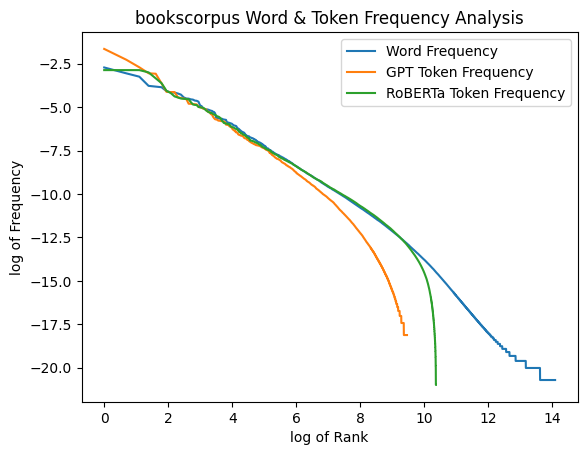
\includegraphics[width=\columnwidth]{../visualizations/bookscorpusfreq.png}
  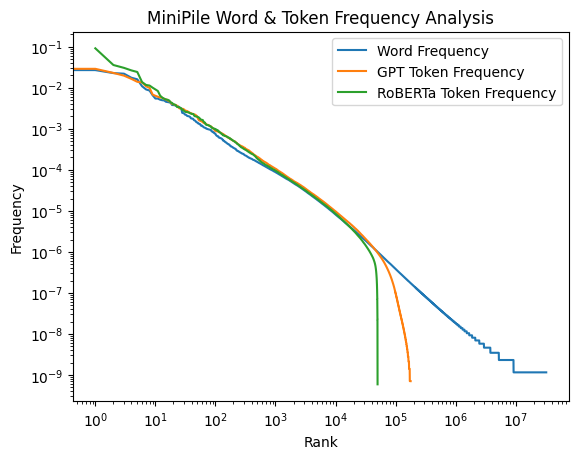
\includegraphics[width=\columnwidth]{../visualizations/minipilecorpusfreq.png}
  \caption{Log-log plots of word \& token rank vs word \& token frequency}
  \label{fig:experiments}
\end{figure}

We also report the least and most common words and tokens for each tokenizer and corpus. We report these words and tokens both including and excluding control tokens and punctuation, which are summarized in Table \ref{tbl:token ranks} and Table \ref{tbl:token ranks no control}.

\begin{table*}
    \centering
    \begin{tabular}{|c|c|c|c|c|c|c|}
        \hline
        \textbf{Rank} & \multicolumn{2}{c|}{\textbf{Word}} & \multicolumn{2}{c|}{\textbf{RoBERTa}} & \multicolumn{2}{c|}{\textbf{GPT-4o}}  \\
        \hline
        1 & . & the & <s> & ␣ & `` & , \\
        \hline
        2 & , & of & \textbackslash n & \textbackslash n & i & ␣the \\
        \hline
        3 & the & and & <\textbackslash s> & . & he & . \\
        \hline
        -1 & restain & RootDir, & seq & ␣Archdemon & wares & aryny \\
        \hline
        -1 & liarliar & homocystinemia & okemon & ␣petertodd & slan & verlening \\
        \hline
        -1 & shop-that & halfday & ython & ␣councill & wier & ␣myx \\
        \hline
    \end{tabular}
    \caption{Summary of most and least common words \& tokens for each corpus, where the left subcolumn is bookscorpus and the right subcolumn is MiniPile, \textit{including} control tokens and punctuation. A rank of -1 indicates a word or token that appears only once in the given corpus. The space character (Unicode U+0020) is denoted by the `␣' character.}
    \label{tbl:token ranks}
\end{table*}

\begin{table}
    \centering
    \begin{tabular}{|c|c|c|c|c|c|c|}
        \hline
        \textbf{Rank} & \multicolumn{2}{c|}{\textbf{Word}} & \multicolumn{2}{c|}{\textbf{RoBERTa}} & \multicolumn{2}{c|}{\textbf{GPT-4o}}  \\
        \hline
        1 & the & the & the & the & i & the \\
        \hline
        2 & to & of & to & of & he & of \\
        \hline
        3 & i & and & and & and & she & and \\
        \hline
    \end{tabular}
    \caption{Summary of most common words \& tokens for each corpus, where the left subcolumn is bookscorpus and the right subcolumn is MiniPile, \textit{excluding} control tokens and punctuation. All of these words are considered \textit{function words} in linguistics literature.}
    \label{tbl:token ranks no control}
\end{table}

We report the $\chi^2$ test statistics for fitted Zipf-Mandelbrot in Table \ref{tbl:kstest}, where we use Equation \ref{eq:zipfmandelbrot} with $a=1.1$ and $b=0$ for all Zipf tests. 

\begin{table*}
    \centering
    \begin{tabular}{|c|c|c|c|}
        \hline
        \textbf{Distribution} & \textbf{Words} & \textbf{RoBERTa} & \textbf{GPT-4o}  \\
        \hline
        bookscorpus & $2.5 \cdot 10^{9}$ & $1.6 \cdot 10^{9}$ & $1.4 \cdot 10^{8}$  \\
        \hline
        MiniPile &  $1.4 \cdot 10^{9}$ & $4.1 \cdot 10^{9}$ & $1.8 \cdot 10^{9}$ \\
        \hline
    \end{tabular}
    \caption{$\chi^2$ test statistics for distribution fit for each tokenizer and corpus, each of which have a p value of near $0$}
    \label{tbl:kstest}
\end{table*}

Finally, we compute the mean squared error (MSE) between the Zipfian prediction and successive applications of a single step of BPE over the Zipfian synthetic dataset in Figure \ref{fig:theoryexperiments}. 

\begin{figure}[t]
  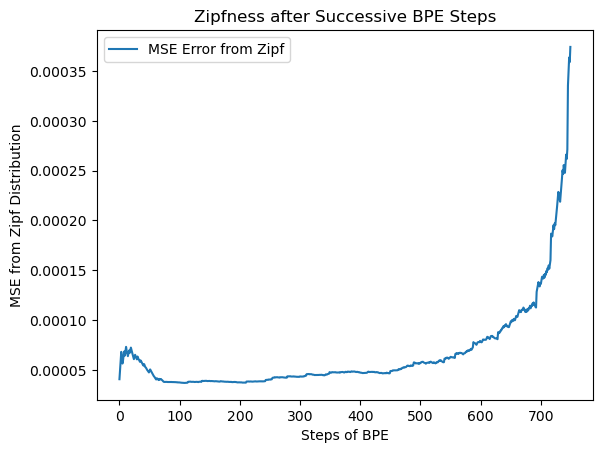
\includegraphics[width=\columnwidth]{../visualizations/zipfnessovertime.png}
  \caption{Mean Squared Error from Zipf prediction of BPE applied to $10^5$ samples of a synthetic Zipf-distributed corpus of $100$ elements}
  \label{fig:theoryexperiments}
\end{figure}

\section{Analysis}

In general, we find strong evidence that BPE tokenizers are Zipfian. Deviations from the Zipfian trend only appear for the final few RoBERTa tokens for both corpuses and the GPT-4o tokens for the MiniPile corpus. This includes in and out-of-distribution text. However, the GPT-4o tokenizer trend on the bookscorpus seems to deviate more dramatically, similar to the multiple regime studies mentioned in Section \ref{section:intro}. We speculate that this may be due to Minipile being a multilingual dataset, which may affect the the distribution for a multilingual tokenizer such as GPT-4o. The $\chi^2$ goodness-of-fit tests confirm a Zipf describes the data well, all having p-values $<<0.0001$. 

Over the token vocabulary, the most common tokens tend to be punctuation, newline characters, and control tokens. Excluding punctuation and special tokens, we recover the known most common English words.

Additionally, applying the BPE pairing process to the synthetic data shows almost no deviations from the original Zipf distribution for hundreds of iterations. However, after about $700$ iterations the MSE from Zipf does begin to increase, though the error is still relatively small.

\section{Conclusions \& Future Work}

The byte pair encoding algorithm, despite building vocabularies using the most frequent pairings of elements, generates vocabularies that are Zipfian, up to the rarest few tokens. We demonstate this over multiple tokenizers and corpuses, including both in and out-of-distribution text. We also provide empirical evidence that Zipfness is preserved over many iterations of BPE.

Noticeable theoretical work has been done to explain Zipf's law for language \cite{li1992}. Most significant was Belevitch's \textit{On the statistical laws of linguistic distributions}\cite{Belevitch1959}, in which the author shows the first order approximation of the rank ordering of many statistical distributions are all Zipfian. This indicates that Zipf's law may be due to the rank ordering of words more than the underlying formation of language. Can Belevitch's proof be shown to be invariant for some number of byte pair encoding transformations?

% Bibliography entries for the entire Anthology, followed by custom entries
%\bibliography{anthology,custom}
% Custom bibliography entries only
\bibliography{custom}

% \appendix

% \section{Example Appendix}
% \label{sec:appendix}

% This is an appendix.

\end{document}